\documentclass[a4paper]{article}

\usepackage[english]{babel}
\usepackage[utf8]{inputenc}
\usepackage{graphicx}
\usepackage{enumitem}
\usepackage{blindtext}

\usepackage{geometry}
\usepackage{textcomp}
\usepackage{pgfplots}

\pgfplotsset{width=10cm,compat=1.9}
\graphicspath{ {./images/} }
    
\title{CS2500 Project 1\\ Merge Sort vs. Insertion Sort}
\author{Evan Wilcox}
\setlength\parindent{0pt}

\newenvironment{myindentpar}[1]%
  {\begin{list}{}%
          {\setlength{\leftmargin}{#1}}%
          \item[]%
  }
  {\end{list}}


\date{Due February 12, 2019}
    
\begin{document}
    \maketitle

    \section{Motivation}
    Sorting is used very often in programs and being able to sort things quickly 
    when needed is extremely important. There is no best sorting algorithm as certain
    algorithms are better in certain situations. Being able to analyse different 
    algorithms to find the best algorithm for a given situation can be very useful.\\

    This report will implement two algorithms in python known as merge sort and 
    insertion sort. The algorithms will then be compared and contrasted by analysing 
    their worst case, best case, and average case run times on varying data sets.


    \section{Background}
    Insertion sort is known to have a asymptotic complexity of $\Theta(n^{2})$ while merge 
    sort has a asymptotic  complexity of $\Theta(n$lg$n)$. Asymptotic  complexity 
    is the run time of an algorithm given a problem size $n$. As $n$ grows increasingly 
    large, an algorithm's run time will increase according to the algorithm's $\Theta()$. \\

    $\Theta()$ is not the only measurement of asymptotic complexity. $\Omega()$ is used to 
    measure an algoritm's best-case run time. Merge sort has a best-case complexity of
    $\Omega(n$lg$n)$ while insertion sort's is $\Omega(n)$. Meaning that as $n$ grows
    increasingly large, an algorithm's run time will perform at least as well as its
    $\Omega()$ times some constant. \\

    Also, $O()$ is used to measure an algorithm's worst-case run time. Insertion sort 
    is known to have a worst-case complexity of $O(n^{2})$ while merge sort has a 
    worst-case complexity of $O(n$lg$n)$. Meaning that as $n$ grows
    increasingly large, an algorithm's run time will perform worse then its $\Omega()$ 
    times some constant. \\

    \textbf{Merge Sort}\\
    Merge sort is a sorting algorithm that sorts by continually splitting the set in 
    half until all elements are in an set of their own, known as divide and conquer.
    It then merges the smaller sets by picking the smallest elements from each set, 
    combining until the entire set is sorted.\\

    Merge sort is often implemented using a technique called recursion. Recursion is the act of calling a 
    function within the function its self on a smaller subset of the problem. 
    Recursion breaks the problem into smaller problems until it can solve the smallest 
    problem called the base case. It then combines the solutions to these smaller 
    problems into the final solution.\\


    \textbf{Insertion Sort}\\
    Insertion sort is a sorting algorithm that iteratively sorts by swapping pairs 
    of elements until the set is sorted. Insertion sort starts at the second element 
    and compares it to the element to its left, if that element is greater it swaps
    the two elements and moves on to the next element, comparing it to all elements
    to its left until it finds one that is not greater than its self. Insertion sort 
    is very similar to how you would sort a hand of cards.

    
    \section{Procedures}
    \begin{enumerate}

        \item Develop a precondition, postcondition, and loop invariants for merge sort
              and insertion sort.
        
        \item Show that the previous preconditions, postconditions, and loop invariants
              are correct.
        
        \item Express merge sort and insertion sort using pseudocode.

        \item Implement merge sort and insertion sort in python.
        
        \item Implement preconditions, postconditions, and invariants using python 
              assert statements to validate correctness.
        
        \item Measure run times of the two algorithms to experimentally determine their
              run time complexity and compare to their expected run time complexity.
        
        \item List problems encountered during development.
        
        \item Develop and implement a testing plan.

        \item Produce a conclusion addressing the efficacy of the methods used.
    \end{enumerate}

    \newpage
    \section{Pseudocode and pre/postconditions}
    
    Insertion Sort Pseudocode
    \begin{verbatim}
    INSERTION-SORT(A)
    1  for j = 2 to A.length
    2    key = A[j]
    3   
    4    i = j - 1
    5    while i>0 and A[i] > key
    6        A[i+1] = A[i]
    7        i = i - 1
    8    A[i+1] = key
    9 
    10 return A\end{verbatim}
    \textbf{Loop Invariant} - Line 1\\
    At the start of each iteration of the for loop on line 1 the subarray A[1..j-1]
    consists of the elements originally in A[1..j-1] but in sorted order.

    \begin{myindentpar}{0.5cm}
        \textbf{Initialization}\\
        Before the for loop j=2 so the subarray A[1..j-1] consists of one element. This
        one element is sorted so the invariant holds.

        \textbf{Maintenance}\\
        The while loop moves A[j] around in the array until it is in sorted order. j is 
        then incremented so the subarray A[1..j] consists of the elements originally 
        in A[1..j] but in sorted order.

        \textbf{Termination}\\
        The condition causing the for loop to terminate is j $>$ A.length. Because j 
        increments by one each iteration we will have j = A.length + 1. Substituting
        A.length + 1 for j in the loop invariant gives us a sorted subarray of
        A[1..A.length] that consists of the elements originally in A[1..A.length] but
        in sorted order. 

    \end{myindentpar}

    \newpage
    Merge Sort Pseudocode
    \begin{verbatim}
    MERGE-SORT(A)
    1 if A.length <= 1
    2     return A
    3 else
    4     m = A.length/2
    5     L = MERGE-SORT(A[1..m])
    6     R = MERGE-SORT(A[m+1..A.length])
    7     return MERGE(L, R)
    \end{verbatim}

    \begin{verbatim}
    MERGE(L, R)
    1  S = []
    2    
    3  while L.length > 0 and R.length > 0
    4      if L[1] < R[1]
    5          S = S + L[1]
    6          L = L[2..L.length]
    7      else
    8          S = S + R[1]
    9          R = R[2..R.length]
    10    
    11 if L.length == 0
    12     S = S + R
    13 else if R.length == 0
    14     S = S + L
    15    
    16 return S
    \end{verbatim}
    
    \textbf{Loop Invariant} - Line 3\\
    At the start of each iteration of the while loop on line 3 the subarray 
    S[1..S.length] consists of elements originally in L and R but in sorted order.

    \begin{myindentpar}{0.5cm}
        \textbf{Initialization}\\
        Before the while loop S is initialized to the empty set []. The array is 
        sorted because it is empty.

        \textbf{Maintenance}\\
        During the while loop, it either removes the first element from L or the first 
        element from R (whichever is less) and adds it to S. Because L and R are sorted,
        elements are being added to S in sorted order so S stays sorted.

        \textbf{Termination}\\
        The condition causing the while loop to continue is L.length $>$ 0 and R.length $>$ 0.
        So, when either of those become false the while loop terminates, meaning, if either 
        L or R are empty the while loop terminates. Because the while loop always removes 
        the first element from L or R, whichever is smaller, either L.length or R.length 
        will equal 0 eventually causing the loop to terminate.

    \end{myindentpar}

    \newpage
    \section{Problems Encountered}
    I had never used python classes before so I had to learn the structure and syntax
    of a python class. Another problem was converting from python 2.x to 3.x because
    I wanted to use a more recent version of python but was used to an older version.

    \section{Testing Plan}
    I plan on testing each algorithm with varying lengths of sorted and unsorted arrays 
    to represent best-case and average-case run time complexities. As well as any edge
    cases such as a zero length array, wrong input types, or arrays of wrong types.

    \vspace{0.5cm}
    \begin{tabular}{ |c|c|c| }
        \hline
        Input             & Expected Output   & Output Recieved   \\ \hline
        Zero length array & Zero length array & Zero length array \\ \hline
        Wrong input type  & Error             & Error caught by precondition checks \\ \hline
        Array of wrong type variables & Error & Error caught by precondition checks \\ \hline
    \end{tabular}

    \section{Performance Results}
    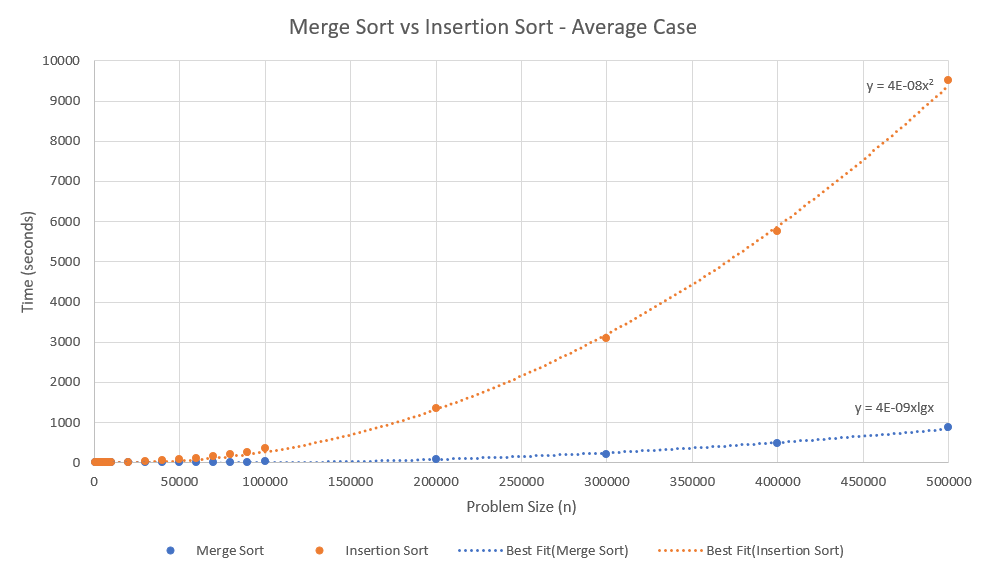
\includegraphics[scale=0.75]{Average}\\

    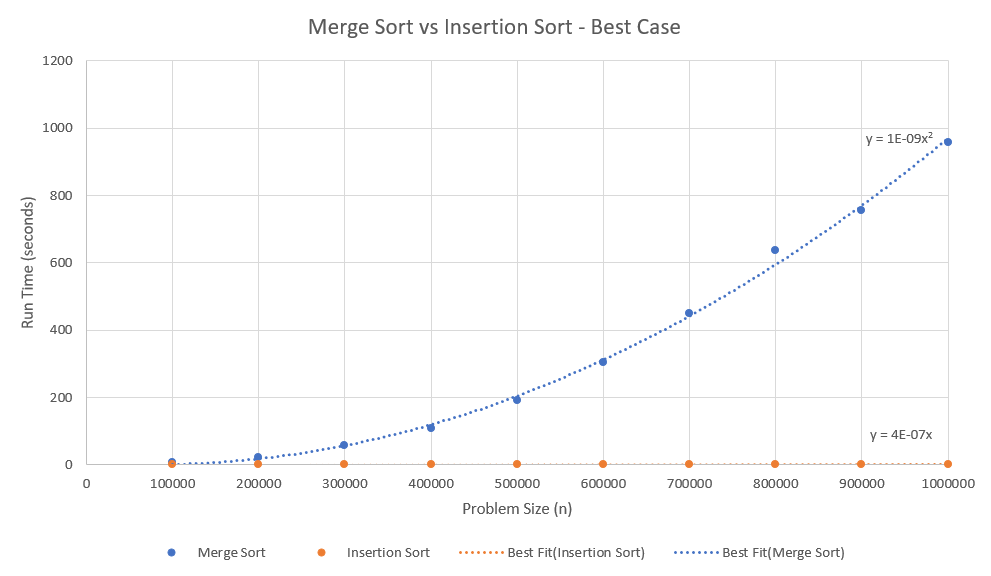
\includegraphics[scale=0.75]{Best}
    
    \vspace{1cm}
    As shown in the first graph, when sorting a random array of integers both Merge
    sort and Insertion sort follow their expected asymptotic complexities of $n$lg$n$
    and $n^{2}$ respectively. Sorting a random array of integers represents the 
    average-case time complexity. As well in the second graph both algorithms follow their 
    expected best-case complexities of $n$lg$n$ and $n$ respectively. Sorting a already 
    sorted array represents the best-case complexity of the algorithms.

    \section{Conclusion}
    In this report we showed that merge sort and insertion sort both follow their expected
    run time complexity measurements. First we showed each algorithm's loop invariants 
    and pre/postconditions then proved they were correct. The algorithms were then
    implemented in a python class to experimentally prove their run time complexities.

    \newpage
    \textbf{Appendix A} - Source Code
    \begin{verbatim}
'''
# @file   proj1.py
# @author Evan Wilcox, CS2500, Section 1A
# @brief  Short program used for experimentally testing merge sort and insertion 
#         sort's expected asymptotic complexity while testing the Sort class's
#         functionality.
''' 

from Sort import Sort
import time, random

sort = Sort()
sort.setDebug(False)

# Used for testing average-case run time.
# Sorts a random array of integers between 0 and n.
for x in [1, 10, 100, 1000, 10000, 100000, 1000000, 10000000]:
    for y in range(1, 10):
        n = x*y
        A = []
        for i in range(0, n):
            A.append(random.randint(0, n))
        
        B = A
        print("N = ", n)
        start = time.time()
        sort.MergeSort(A)
        print("Merge Sort     = ", time.time()-start)
        start = time.time()
        sort.InsertionSort(B)
        print("Insertion Sort = ", time.time()-start, "\n")
        
# Used for testing best-case run time.
# Sorts a sorted array of integers between 0 to n.
for x in [1, 10, 100, 1000, 10000, 100000, 1000000, 10000000]:
    for y in range(1, 10):
        n = x*y
        A = []
        for i in range(0, n):
            A.append(i)
        
        print("N = ", n)
        start = time.time()
        sort.MergeSort(A)
        print("Merge Sort     = ", time.time()-start)
        start = time.time()
        sort.InsertionSort(A)
        print("Insertion Sort = ", time.time()-start, "\n")
    \end{verbatim}

    \begin{verbatim}
'''
# @file   Sort.py
# @author Evan Wilcox, CS2500, Section 1A
# @brief  A class wrapper for Merge Sort and Insertion Sort.
''' 

'''
# @class Sort
# @brief A class wrapper for Merge Sort and Insertion Sort.
''' 
class Sort:
    '''
    # @fn    __init__
    # @brief Class initializer.
    # @pre   No pre-condition.
    # @post  A Sort object is created.
    ''' 
    def __init__(self):
        self.debug = False      # indicates whether debug mode is enabled.
    
    '''
    # @fn    setDebug
    # @brief Sets the debug mode on or off.
    # @pre   val must be a boolean
    # @post  The new debug mode is set.
    # @param val new intended debug mode
    ''' 
    def setDebug(self, val):
        # Precondition
        if self.debug:
            assert type(val) == bool
        
        self.debug = val
    
    '''
    # @fn     MergeSort
    # @brief  Sorts the given array using Merge Sort.
    # @pre    A must be an array of integers.
    # @post   A is sorted.
    # @param  A an array containing integers.
    # @return A sorted array of integers.
    '''
    def MergeSort(self, A):
        # Precondition
        if self.debug:
            assert type(A) == list
            for i in range(len(A)):
                assert type(A[i]) == int
        
        if len(A) <= 1:
            return A
        else:
            m = int(len(A)/2)
            L = self.MergeSort(A[0:m])
            R = self.MergeSort(A[m:])
            
            # Postcondition
            if self.debug:
                assert self.checkSort(self.merge(L, R))
            
            return self.merge(L, R)

    '''
    # @fn     merge
    # @brief  Merges two sorted arrays in to one sorted array.
    # @pre    Both L and R must be arrays of integers in sorted order.
    # @post   L and R are merged in to one sorted array.
    # @param  L An array of sorted integers.
    # @param  R An array of sorted integers.
    # @return An array of sorted integers.
    ''' 
    def merge(self, L, R):
        # Preconditions
        if self.debug:
            assert type(L) == list
            assert type(R) == list
            
            for i in range(len(L)):
                assert type(L[i]) == int
                
            for i in range(len(R)):
                assert type(R[i]) == int
        
            assert self.checkSort(L)
            assert self.checkSort(R)

        S = []
        '''
        # loop description while loop that merges two arrays 
        # invariant:       S consists of elements from L and R in sorted order
        # proof:           
        # initialization:
        #    S is initialized to [] so it is sorted.
        #
        # maintenance: 
        #   The first element is removed from L or R and added to
        #   S. Because L and R are sorted S stays sorted.
        #
        # termination:
        #   Because an element is always removed from L or R either
        #   L or R size will equal 0 so the while loop will terminate.
        ''' 
        while len(L) > 0 and len(R) > 0:
            # Invariant
            if self.debug:
                assert self.checkSort(S)
            
            if L[0] < R[0]:
                S.append(L[0])
                L = L[1:]
            else:
                S.append(R[0])
                R = R[1:]
        
        if len(L) == 0:
            S = S + R
        elif len(R) == 0:
            S = S + L
        
        # Postcondition
        if self.debug:
            assert self.checkSort(S)
        
        return S


    '''
    # @fn     InsertionSort
    # @brief  Sorts the given array using Insertion Sort.
    # @pre    A must be an array of integers.
    # @post   A is sorted.
    # @param  A an array containing integers.
    # @return A sorted array of integers.
    ''' 
    def InsertionSort(self, A):
        # Preconditions
        if self.debug:
            assert type(A) == list
            for i in range(len(A)):
                assert type(A[i]) == int
        '''
        # loop description iterates through elements in the array
        # invariant:       A[1..j-1] consists of elements originally in A[1..j-1]
        #                  but in sorted order.
        # proof:           
        # initialization:
        #    Before the loop j=2 so the subarray A[1..j-1] contains 1 element. 
        #
        # maintenance: 
        #   The while loop moves A[j] around until it is in sorted order. j is incremented
        #   so the subarray A[1..j] is in sorted order.
        #
        # termination:
        #   The terminating condition is j > A.length, at this time j = A.length + 1. 
        #   Subsitute that in to the invariant and the subarry A[1..A.length] contains
        #   elements originally from A[1..A.length] but in sorted order.
        ''' 
        for j in range(1, len(A)):
            # Invariant
            if self.debug:
                assert self.checkSort(A[0:j])
            
            key = A[j]
            i = j - 1

            while i >= 0 and A[i] > key:
                if self.debug:
                    assert self.checkSort(A[0:i])
                
                A[i + 1] = A[i]
                i = i - 1
            A[i + 1] = key
        
        # Postcondition
        if self.debug:
            assert self.checkSort(A)
        
        return A


    '''
    # @fn     checkSort
    # @brief  Checks if the given array A is in sorted order.
    # @pre    A must be an array on integers.
    # @post   A boolean is returned.
    # @param  A an array of integers.
    # @return Boolean indicating if the passed array is sorted in 
                increasing order.
    ''' 
    def checkSort(self, A):
        # Preconditions
        if self.debug:
            assert type(A) == list
            for i in range(len(A)):
                assert type(A[i]) == int
        
        for i in range(0, len(A)-1):
            if A[i] > A[i+1]:
                return False

        return True
    \end{verbatim}

\end{document}